\chapter{Estado da Arte} \label{chap:sota}

\section{Arquiteturas de Redes UAV}\label{sec:architectures}

Dependendo do contexto em que estão inseridos, os UAVs podem estar dispostos e ser controlados de diversas formas. Ao longo desta secção serão analisadas diferentes arquiteturas de redes UAV, o modo como funcionam e a maneira comoos UAVs interagem  entre si e em rede.

\subsection{Controlo Directo}
Neste tipo de arquitetura, cada UAV é controlado diretamente pela sua estação controladora fazendo com que não exista qualquer tipo de interação inter-UAV. Sendo que cada comando é enviado diretamente para cada UAV e sendo executado apenas pelo próprio como demonstrado na figura \ref{fig:controlo_directo}.

\begin{figure}[H]
\centering
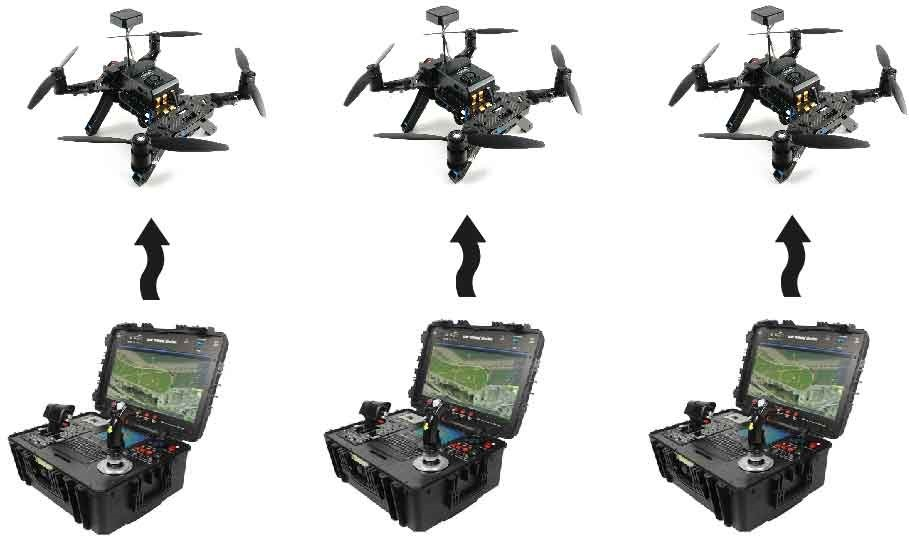
\includegraphics[width=60mm]{controlo_direto}
\caption{A arquitectura de controlo directo \label{fig:controlo_directo}}
\end{figure}

As GCSs podem ser implementadas de diferentes formas: podem ser implementadas através de uma antena Wi-Fi, que distribui o sinal de comando para os UAVs, ou então, numa versão mais simples através de telecomando sendo que esta é opção a mais utilizada em captação de imagem e vídeo.

No entanto, como esta arquitectura é baseada num modelo de controlo mais centralizado possui algumas desvantagens tais como: 

\begin{itemize}
\item Se houver um ponto de falha, o sistema fica comprometido;
\item Nem todos os UAVs estão ligados à GCS a todo o instante, e assim sendo, os sinais de controlo podem não chegar ao drone;
\item E por fim, pode constituir um problema não só para comunicação mas também, para a segurança do sistema \cite{ImadJawhar2017}.
\end{itemize}

\subsection{Enxames de UAVs}

Um enxame de UAVs é capaz de formar redes expansíveis, para além das infraestruturas, que permitem o acesso dos nós terrestres. Ao beneficiar dos recursos de alta flexibilidade e de rápida provisão, a \textit{swarm} de UAVs é uma solução viável para recuperar a comunicação de forma rápida e eficaz, especialmente em cenários onde os recursos de comunicação são escassos ou inexistentes, como nos ambientes pós-desastre \cite{Shi2018}. 

Nesta arquitetura, as ligações d2d, \textit{drone-to-drone} são necessárias para fazer a comunicação entre os UAVs existentes no enxame. Num enxame, existe uma hierarquia que é constituída por um líder e pelos seguidores. O líder é o UAV que recebe os comandos, e os seguidores são os que seguem a rota do líder e os comandos que lhe são passados por este.

\begin{figure}[H]
\centering
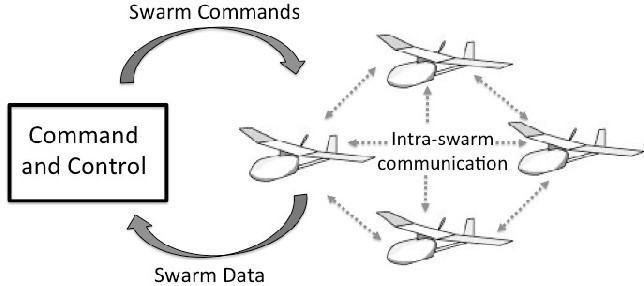
\includegraphics[width=10cm]{uav_swarm}
\caption{Diagrama de Controlo e Comando de um enxame UAV\label{fig:uav_swarm} }\cite{G.Madey2013}
\end{figure}

Esta topologia suporta não só a troca de mensagens de controlo entre os UAVs, de modo a prevenir colisões e a calcular rotas de voo,  bem como a transmissão dos dados para serem acedidos por outros UAVs. Existem UAVs específicos dentro do enxame que estão equipados com interfaces para comunicar com as infraestruturas ou satélites, estes estabelecem as \textit{gateways} entre o enxame e as outras redes.

Nos meios rurais ou nos meios de pós-desastre onde as infraestruturas de cobertura são escassas, os enxames UAV são formados como infraestruturas aéreas temporárias de acesso para os veículos de apoio a esses meios \cite{Shi2018}.

No exemplo citado no artigo \cite{He2018}, é estudada a possibilidade de um enxame de UAVs através do algoritmo proposto contar com vários líderes mas também, ao longo do tempo haver a possibilidade de aumentar o número de seguidores, a fim de reduzir o consumo de comunicação e melhorar a adaptabilidade do sistema e também a sua expansibilidade.

\subsection{Redes \textit{Mesh}}

Uma rede \textit{mesh} sem fio consiste em nós de rádio organizados numa topologia \textit{mesh} ou malha. Estas redes são normalmente compostas por \textit{routers} e \textit{gateways mesh} que distribuem o sinal de \textit{Wi-Fi} igualmente por todos os pontos da rede.

Nestes cenários de rede, os \textit{routers} comunicam entre si e enviam sinal \textit{Wi-Fi} reciprocamente, bem como, para a área envolvente. Por exemplo, se um nó A quiser comunicar com o nó C irá utilizar o nó B que fica entre ambos para fornecer melhor possibilidade de comunicação. 

À transmissão de informação entre os nós passando por este meio de um nó intermediário (nó B), dá-se o nome de “salto” ou “\textit{hop}” da rede mesh. Cada um destes \textit{hops} introduz um nível de atraso na rede por isso, é necessário que o número de saltos seja minimizado encontrando por exemplo o caminho mais direto entre os dois nós. No entanto, quando um dos \textit{routers} da rede \textit{mesh} fica \textit{offline} ou inutilizado o sinal consegue encontrar outros caminhos graças aos nós alternativos \cite{NetSpot}.

Nesta configuração de rede mesh encontra-se o projeto UAVNet referenciado no artigo \cite{Morgenthaler2012a}, que é uma \textit{framework} baseada numa altamente adaptável \textit{wireless mesh network}, WMN, que faz uso de UAVs pequenos equipados com \textit{wireless mesh nodes}, conectados aos UAV via porta série, de modo a poder interagir como uma \textit{mesh} em pleno ar.

\begin{figure}[H]
\centering
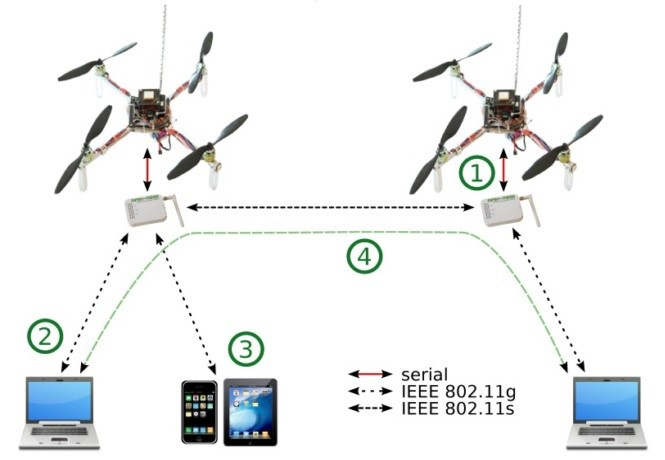
\includegraphics[width=10cm]{uav_net}
\caption{Exemplo de aplicação do \textit{UAVNet} \label{fig:uav_net} }\cite{Morgenthaler2012a}
\end{figure}

\subsection{Redes Ad-Hoc}

A tecnologia \textit{ad-hoc} permite a criação de redes de dispositivos móveis em áreas onde não existem infraestruturas de comunicações. Neste tipo de ligação, não existe um nó central para onde todas as informações são enviadas pelos outros nós, fazendo com que não seja necessária a existência de um \textit{router} que faça a comunicação da rede com outros dispositivos externos. As ligações entre nós são independentes entre si, de maneira que, se uma falhar, seja por perda de conexão ou falha de algum dispositivo, todas as outras ligações continuam a funcionar \cite{DalloraMoraes2007}.

Como as redes \textit{ad-hoc} funcionam sem nenhuma infraestrutura é necessário que existam mecanismos de descoberta de rotas e encaminhamento de informação. Para isso, estas redes recorrem a protocolos de rotas de dois tipos: os reativos e os pró-ativos.

Dentro dos protocolos reativos, que são protocolos que não tomam iniciativa de manter as rotas e apenas as determinam, quando necessário, fazendo \textit{flooding} de pedidos na rede. Este protocolo tem como vantagem o facto de usar recursos apenas quando é necessário, no entanto, inundam a rede com pedidos e introduzem atraso no inicio de envio do tráfego pois tem de ser primeiramente determinada a rota. Neste tipo de protocolos inclui-se o AODV definido pela norma RFC 3561, onde um determinado nó A envia um \textit{Route Request} para poder efetuar a comunicação com o nó B e recebe deste um \textit{Route Reply} de forma a indicar a rota mais próxima.

No caso dos protocolos pró-ativos, as rotas são construídas utilizando tráfego de controlo contínuo e mantidas todas as rotas. Este processo tem como vantagem ter as rotas sempre disponíveis e mantém o tráfego de controlo constante. Um exemplo deste tipo de protocolo é o OLSR definido pela norma RFC 3626. Este protocolo implementa um sistema de deteção de ligação a nós vizinhos, através de mensagens \textit{HELLO} que efetuam os pedidos de encaminhamento de forma otimizada através do mecanismo de MPR. Para além destes dois aspetos este protocolo envia mensagens de estado das ligações e cálculo de rotas \cite{Ricardoa}.

Em relação aos drones existem estudos sobre as FANETs, que são redes \textit{ad-hoc} constituídas por UAVs, como se pode comprovar através do artigo \cite{Bekmezci2013a}. Um dos exemplos de rede ad-hoc com equipamentos UAV é o que está referenciado no artigo \cite{Brown2004} que fala de dois cenários de funcionamento, no primeiro o UAV atua como um nó de rádio proeminente que efetua a conexão de dos pontos de rádio terrestres desativados. No segundo cenário, a rede permite que os grupos de UAVs comuniquem entre si para estender o alcance operacional dos UAVs mais pequenos.

\begin{figure}[H]
\centering
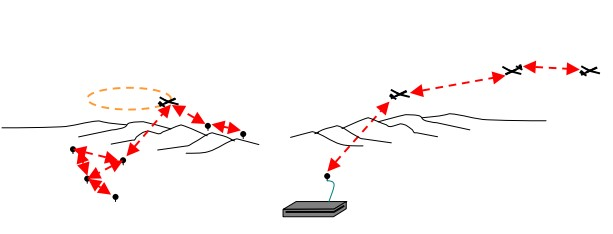
\includegraphics[width=10cm]{ad-hoc_protocols}
\caption{Figuras ilustrativas do cenário 1 (esquerda) e do cenário 2 (direita)  \label{fig:ad-hoc_protocols}}
\cite{Ricardoa}
\end{figure}

\subsection{Redes SD-UAV}

As redes definidas por software (SDN) são o novo paradigma de \textit{networking} no qual o \textit{hardware} de encaminhamento é dissociado das decisões de controlo. É uma tecnologia que promete simplificar a gestão da rede e permitir a inovação e evolução. A ideia principal é permitir que os software developers confiem nos recursos de rede da mesma maneira que fazem com os recursos de armazenamento e computação. Nas SDN, a inteligência da rede é centralizada logicamente nos controladores baseados em \textit{software} (plano de controlo) e os dispositivos de rede tornam-se simples dispositivos de encaminhamento de pacotes (plano de dados) que podem ser programados através de uma interface aberta \cite{Nunes2014} (ex. OpenFlow \cite{Leon-Garcia2015}, etc).

No artigo \cite{Secinti2018} é proposto um protocolo de gestão de uma rede aérea contruído em cima de uma arquitetura SDN. Neste projeto cada UAV torna-se num switch SDN que é controlado por comandos enviados por um controlador centralizado.

\begin{figure}[H]
\centering
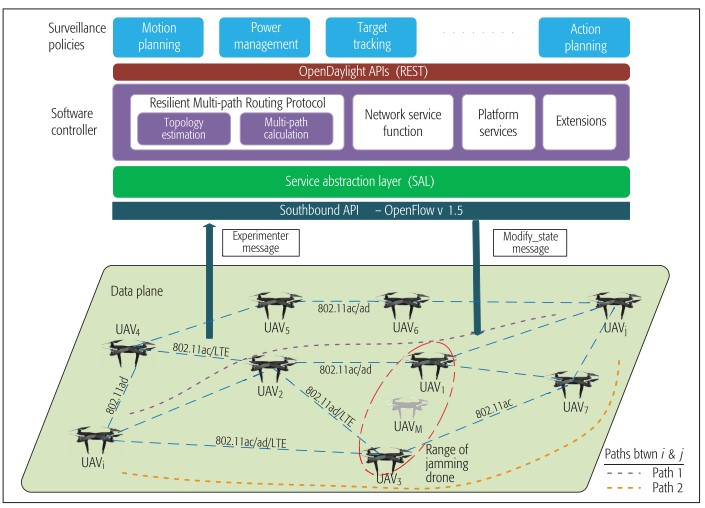
\includegraphics[width=10cm]{sd-uav_architecture}
\caption{Arquitetura SD-UAV proposta no artigo  \label{fig:sd-uav_architecture} }\cite{Secinti2018}
\end{figure}



\section{Áreas de aplicação das redes UAV}\label{sec:application}

Tal como dito em cima na secção \ref{sec:context}, os UAV e as suas redes tem várias utilidades tais como: escoltas militares, troca de mercadorias em algumas cidades, gestão do trânsito, fotografia aérea e segurança urbana. No entanto existem outros serviços e aplicações em que estas podem operar.

\subsection{Retransmissão de Comunicação}

Os UAVs podem funcionar como nós de retransmissão que conectam \textit{clusters} desconectados da rede \textit{ad hoc} móvel (MANET).  Nesse caso, os nós pertencentes a diferentes \textit{clusters} podem comunicar entre si utilizando um UAV, que pode ser colocado numa posição estratégica entre os dois. Por essa questão, um ou mais UAVs podem fornecer essa função em grandes MANETs, proporcionando eficiência de comunicação e flexibilidade. Adotando essa estratégia, pode estender-se uma MANET numa área geográfica muito grande, onde os nós podem ter que ser agrupados em diferentes regiões devido aos requisitos de topologia de terrenos, localização de nós e mobilidade impostos pelo aplicação \cite{ImadJawhar2017}.

\subsection{Gateways de Rede}

Em áreas geográficas remotas ou áreas atingidas por desastres, um ou mais UAVs podem fornecer conectividade a redes de \textit{backbone}, infraestrutura de comunicação ou acesso à Internet agindo como nós de \textit{gateway}. Essa função pode desempenhar um papel essencial para restaurar a cobertura de telefone, internet ou satélite desesperadamente necessária nesses locais. Essa conectividade pode apoiar esforços de busca e salvamento de vidas e reconstrução. Os UAVs podem ser implantados de maneira rápida e eficiente para executar essa tarefa de maneira muito dinâmica e económica \cite{ImadJawhar2017}.

\subsection{UAV-assisted Sensing}

As várias aplicações requerem vários UAVs de colaboração para efetuar a deteção de uma área ou inspecionar uma infraestrutura utilizando um ou vários tipos de sensores como câmaras fotográficas, sensores de calores, leitores de radiação e monitores de gás. Essas aplicações exigem uma eficiência grande de comunicação de modo a permitir uma melhor deteção entre os vários UAVs. Alguns dos UAVs podem individualmente lidar com algumas das tarefas de deteção. Uma solução eficiente para este problema passa por usar vários UAVs juntos na organização das operações e fazer uma colheita coletiva de informações mais precisas e confiáveis \cite{ImadJawhar2017}

\subsection{UAV-assisted Acting}

Em alguns casos, como fins agrícolas e militares, exigem dispositivos atuadores, como os UAVs. Nesse tipo de aplicações, vários UAVs podem colaborar entre si para realizar as tarefas necessárias. No caso da agricultura, vários UAVs poderiam trabalhar juntos para realizar a pulverização de grandes campos com pesticidas ou fazer distribuição rápida de sementes em grandes áreas \cite{ImadJawhar2017}.

\subsection{UAV-based data storage}

Apesar de algumas aplicações de UAVs enviarem os dados recolhidos diretamente para a estação base, outros podem necessitar que os UAVs armazenem a recolha de dados devido a três grandes motivos. A primeira é que os dados recolhidos necessitam de grande largura de banda de comunicação e os dados podem não estar sempre disponíveis para a transferência dos UAVs para a estação base. A segunda razão é que não existe a necessidade de enviar os dados recolhidos imediatamente para a estação logo após a recolha, pois a informação será usada e processada após a recolha. A terceira razão é que os dados recolhidos precisam de ser transferidos para a estação base somente após os dados serem processados e agregados instantaneamente durante a operação. Os UAVs podem ser homogéneos ou heterogéneos em termos de capacidade de armazenamento e capacidade de recolha de dados. Os UAVs podem recolher quantidades iguais ou diferentes de dados, dependendo claro do tipo de aplicação \cite{ImadJawhar2017}.

\subsection{UAV-based data processing}

Os UAVs podem ser equipados com unidades de processamento de última geração que podem ser utilizados por UAVs colaborativos para aplicações que precisam de processamento de alto desempenho, como processamento de imagem de alta resolução, processamento de vídeo, reconhecimento de padrões, fluxo de dados e planeamento de tarefas online. Uma tarefa de processamento de dados de alto desempenho pode ser obtida utilizando uma unidade computorizado num UAV ou várias unidades computorizadas disponíveis em vários UAVs. Neste último caso, precisa de ser efetivamente utilizada a abordagem de processamento distribuído pelos processadores disponíveis. Isto é geralmente muito importante se os UAVs estiverem a operar em zonas distantes das estações base e quando os resultados forem necessários no momento para acionar uma opção adequada. Por exemplo, num campo de batalha, um UAV pode precisar de identificar uma unidade inimiga que esteja próxima de algumas das suas unidades. Nesse caso o processamento de imagens e o reconhecimento de padrões são necessários para localizar o inimigo e tentar destruí-lo \cite{ImadJawhar2017}.

\section{Software de Controlo Open-Source}\label{chap:cs_opensource}

Nesta secção será analisada informação relativa tanto a \textit{software} e protocolos \textit{open source} existentes no mercado e que poderão a vir a ser utilizados na solução implementada.

\subsection{Papparazzi UAV}

O projeto Paparazzi UAV, fundado em 2003, é um projeto open source de hardware e software que abrange tanto a parte de software da estação terrena como os sistemas de pilotagem autónoma para os vários tipos de drones. Este projeto tem como principal foco o voo autónomo e o voo manual como um objetivo secundário \cite{TheFr2003}

\subsubsection{Arquitecturas Implementadas}

A nível das arquiteturas abordadas na secção acima este software é capaz de suportar todas as arquiteturas demonstradas acima com exceção das redes SD-UAV uma vez que ainda se encontra em fase de estudos. Estas implementações podem ser comprovadas nos artigos \cite{Remes2013,Bouachir2014a}.

\pagebreak
\subsubsection{Áreas de Aplicação}
Este software integra varias áreas de aplicação no entanto, as que mais se destacam nesta tecnologia são as seguintes:

\begin{itemize}
    \item Rede de Sensores;
    \item Investigação científica;
    \item Processamento de dados;
\end{itemize}

\subsubsection{Funcionalidades Protocolares de Comunicação e de Controlo}

A nível de funcionalidades protocolares de comunicações e controlo o Paparazzi UAV trabalha com alguns dos mais recentes protocolos de comunicação como o \textit{ZigBee(Xbee)}, \textit{Wi-Fi} e \textit{Bluetooth}\cite{TheFr2003}.

\subsection{ArduPilot}
O \textit{ArduPilot} é uma tecnologia que visa permitir a criação e o uso de sistemas de veículos não tripulados confiáveis e autónomos para o benefício pacífico de todos. É um projeto que atualmente pode ser descrito como uma \textit{suite} para um piloto automático \cite{ArduPilotCommunity}.

\subsubsection{Arquitecturas Implementadas}

As arquiteturas suportadas por esta tecnologia são as seguintes: controlo direto, enxames e também com mesh encontrando-se as áreas de ad-hoc e SD-UAV ainda em fase de desenvolvimento.

\subsubsection{Áreas de Aplicação}

Entre as áreas de aplicação desta tecnologia encontram-se:
\begin{itemize}
    \item {Mapeamento Aéreo;}
    \item Procura e Salvamento VTOL;
    \item Agricultura com os tratores automáticos;
    \item Controlo de veículos submarinos.
\end{itemize}

\subsubsection{Funcionalidades Protocolares de Comunicação e de Controlo}

A este nível de funcionalidades protocolares esta tecnologia é um pouco mais completa que a tecnologia apresentada anteriormente já que suporta não só o protocolo \textit{Wi-Fi} mas também suporta as tecnologias:
\begin{itemize}
    \item \textit{MAVLink} - é um protocolo de mensagens \textit{lightweight} para comunicação com drones (e entre componentes \textit{onboard} do drone). Segue um padrão de \textit{design} moderno híbrido de \textit{publish-subscriber} e ponto-a-ponto \cite{DronecodeProject}.
    \item CAN - \textit{Controller Area Network}
    \item UAVCAN - é um protocolo leve projetado para comunicação confiável em aplicações aeroespaciais e robóticas pelo barramento CAN \cite{UAVCANdevelopmentteam}.
\end{itemize}

\subsection{Dronecode}

A tecnologia Dronecode apresenta-se como uma solução \textit{full-stack} para os \textit{drones}, com soluções que vão desde a estação de controlo, GCS, até ao próprio \textit{drone} e aos seus sensores. Esta tecnologia criada sob a alçada da Fundação \textit{Linux} e que tem como objetivo promover o desenvolvimento dos drones contando com parceiros tais como a \textit{Qualcomm} e a \textit{Intel} \cite{DronecodeProject}.

\subsubsection{Arquitecturas Implementadas}

A nível de arquiteturas esta tecnologia é também uma das mais completas, tendo em conta os objectivos do projeto \textit{Dronecode} que é como diz em cima ser um dos parceiros para o desenvolvimento dos \textit{drones}. Por isso, esta tecnologia está apta a trabalhar com todas as arquiteturas referidas na secção \ref{sec:architectures}. 

\subsubsection{Áreas de Aplicação}

Nesta tecnologia as áreas de aplicação abrangidas são vastas, entre as quais destacam-se as seguintes:

\begin{itemize}
    \item Carga e Entrega - de pequenos pacotes como medicamentos;
    \item Inspeções aéreas - como por exemplo, mapeamento geográfico, inspeções em canteiros de obras e gasodutos, gestão da vida selvagem, gestão de fazendas etc;
    \item Entretenimento - competições e afins;
    \item Fotografia aérea;
    \item Busca, Salvamento e fiscalização - fiscalização de fronteiras;
    \item Exploração e Investigação - para fins académicos e científicos \cite{DronecodeProject}.
\end{itemize}

\subsubsection{Funcionalidades Protocolares de Comunicação e de Controlo}

A nível de funcionalidades protocolares de comunicação esta tecnologia utiliza também algumas das que já foram abordadas noutas tecnologias descritas em cima. Entre essas tecnologias estão o \textit{Wi-Fi}, o \textit{MAVLink} e o UAVCAN. Para além destas duas há ainda a destacar o RTPS, neste caso FastRTPS \cite{DronecodeProject}. O protocolo de comunicação RTPS que é uma \textit{framework publish subscrive} de alta performance que partilha a informação nos sistemas distribuidos utilizando um modelo desacoplado que se baseia em \textit{Publishers}, \textit{Subscrivers} e \textit{Data Topics}\cite{EProsima}.

\subsection{LibrePilot}

O projecto \textit{open source} LibrePilot foi fundado em 2015. Este projecto foca-se na investigação e desenvolvimento de \textit{hardware} e \textit{software} para serem utilizados numa variedade de aplicações incluindo controlo de e estabilização veículos , UAVs e \textit{robots}. Um dos principais objectivos do projecto é conseguir arranjar um ambiente aberto e colaborativo e fazer dele a casa ideal para o desenvolvimento de ideias inovadoras \cite{LibrePilot}.

\subsubsection{Arquitecturas Implementadas}

Segundo a documentação desta tecnologia esta está mais virada para a arquitetura de controlo directo, focando-se muito na interação com \textit{smartphones} como estações de controlo através de uma \textit{app Android} que se encontra disponível \textit{online}\cite{LibrePilot}.

\subsubsection{Áreas de Aplicação}

Esta tecnologia não é muito basta em termos de áreas de aplicação uma vez que na sua documentação e em foruns utilizados pela comunidade de \textit{developers} apenas é referida a sua utilização para fotografia aérea \cite{LibrePilot}.

\subsubsection{Funcionalidades Protocolares de Comunicação e de Controlo}

Nas funcionalidades de comunicação e controlo para esta tecnologia encontra-se o protocolo \textit{MAVLink} já referida nesta secção e para além disso suporta também o protocolo MSP, que é um protocolo de comunicação desenvolvido pela \textit{MultiWii} desenhado para ser leve, genérico, eficiente e seguro \cite{MultiWii,MultiWiiForum}. 

\subsection{Comparação de soluções}

Nesta secção será disponibilizada uma tabela comparativa de todas as soluções apresentas nas sub-secções em cima.


%%%%%%%TABELA 1%%%%%%%%%%%%%%%%%%%%%%%%%%%%%%%%%%%%%%%%%%%%%%%%%%%%%%%%%%%%%%%%%%%%%%%
\begin{table}[H]
\caption{Comparação das várias opções de \textit{software}}
\begin{tabular}{l|c|c|c|}
\cline{2-4}
& \multicolumn{1}{l|}{Arquiteturas}  & \multicolumn{1}{l|}{Protocolos}  & \multicolumn{1}{l|}{Documentação} \\ \hline
\multicolumn{1}{|l|}{PapparazziUAV} & \textit{CD, SW, Mesh e Ad-Hoc}  & \textit{Xbee, Wi-Fi e Bluetooth} & Razoável \\ \hline
\multicolumn{1}{|l|}{ArduPilot}     & \textit{CD, SW, Mesh, Ad-Hoc e SD-UAV} & \textit{MAVLink, WiFi, CAN e UAVCAN}      & Boa                               \\ \hline
\multicolumn{1}{|l|}{Dronecode}     & Todas                                  & \textit{MAVLink, WiFi, UAVCAN e FastRTPS} & Muito Boa                         \\ \hline
\multicolumn{1}{|l|}{LibrePilot}    & CD                       & \textit{MAVLink e MSP}                    & Razoável                          \\ \hline
\end{tabular}
\end{table}
%%%%%%%%%%%%%%%%%%%%%%%%%%%%%%%%%%%%%%%%%%%%%%%%%%%%%%%%%%%%%%%%%%%%%%%%%%%%%%%%%%%%%%%%%%%%%%%%%